\chapter{Desarrollo}

\section{Preparación de los datos}

\subsection{Obtención de los datos}

Esta sección describe cómo se han obtenido los datos del proyecto. Primero se presenta la fuente de datos utilizada y su estructura, y después se explica el proceso de descarga y construcción del dataset.

\subsubsection{Fuente de datos}

La fuente de datos principal utilizada para la realización de este trabajo es StatsBomb Open Data, un repositorio público disponible en GitHub que proporciona conjuntos de datos e investigaciones para mejorar la comprensión del fútbol.

Los datos de este repositorio están estructurados en tres niveles jerárquicos.
\begin{itemize}
    \item \textbf{Competiciones} (\texttt{data/competitions.json}), que contiene el catálogo completo de competiciones y temporadas disponibles. Entre los campos que incluye cada entrada destacan el identificador de la competición (\texttt{competition\_id}), el identificador de la temporada (\texttt{season\_id}), el nombre de la competición, el nombre de la temporada y el género de la competición, entre otros.

    \item \textbf{Partidos} (\texttt{data/matches/\{competition\_id\}/\{season\_id\}.json}), que contiene los metadatos de todos los partidos de una competición y temporada concretas. Entre los campos disponibles en cada entrada destacan el identificador del partido (\texttt{match\_id}), los equipos local y visitante, el marcador final, la fecha, la jornada, el estadio, el árbitro y el estado del partido, entre otros. Solo los partidos con estado \textit{available} tienen fichero de eventos asociado y han sido incluidos en el dataset.

    \item \textbf{Eventos} (\texttt{data/events/\{match\_id\}.json}), que contiene el registro completo de acciones de un partido, ordenadas cronológicamente. Cada acción incluye el tipo de evento, el equipo, el minuto y segundo de juego, la localización en el campo y los atributos específicos del tipo de acción. Es el fichero principal del que se extrae la información para construir el dataset de modelado.
\end{itemize}

El repositorio también incluye otros ficheros de alineaciones y datos de posicionamiento 360° que no se utilizan en este trabajo ya que no son necesarios para el enfoque planteado. La especificación técnica completa de los campos de cada tipo de fichero está recogida en la carpeta \texttt{doc/} del repositorio, con documentos específicos para competiciones, partidos y eventos.

\subsubsection{Proceso de descarga y construcción del dataset}

El dataset utilizado para este proyecto se ha construido utilizando un script de Python que automatiza la descarga y el almacenamiento de los datos del repositorio StatsBomb Open Data.

El primer paso para generar este dataset consiste en descargar el catálogo de competiciones y para competición se descarga el fichero de partidos disponibles. Por cada partido, se obtiene el fichero de eventos correspondiente y se itera sobre cada acción registrada. Para cada evento se extrae un conjunto de campos comunes y unos campos específicos según el tipo de acción. Cada acción pertenece a una fila del dataset. Al ejecutar este script, se obtiene un fichero csv con todos los eventos de cada partido disponible. La columna \texttt{final\_result}, derivada del marcador final de cada partido, actúa como etiqueta de clasificación y toma los valores \texttt{home\_win}, \texttt{draw} o \texttt{away\_win} según si el equipo local ganó, empató o perdió.

Dado que el proceso implica miles de peticiones a un servidor externo, se han tomado algunas medidas para hacerlo más resistente a fallos de red. Ante un error de descarga, el script reintenta la petición hasta tres veces con pausas progresivas de 5, 10 y 15 segundos antes de registrar el fallo. Para evitar perder el trabajo acumulado en caso de un error tardío, el dataset se guarda de forma parcial al terminar cada competición. Por último, se ha implementado una función de verificación que cruza los partidos del dataset con los disponibles en el repositorio y genera automáticamente el comando necesario para recuperar cualquier partido que falte.

\subsection{Comprensión y análisis de los datos}

\subsubsection{Estructura del dataset}

El dataset resultante es un fichero tabular con 12.188.949 filas y 28 columnas, donde cada fila representa un evento individual registrado durante un partido. El conjunto abarca 3.464 partidos de 21 competiciones distintas, que incluyen ligas masculinas de élite, competiciones femeninas y torneos internacionales.

La densidad de eventos es consistente entre partidos, con una media de 3.519 eventos por partido, un mínimo de 2.101 y un máximo de 5.190. Esta regularidad indica que no existen partidos con registros incompletos o truncados que pudieran introducir ruido en las métricas acumuladas.

\subsubsection{Tipos de evento}

El dataset contiene 33 tipos de evento con una distribución muy desigual. Los tres más frecuentes (\textit{Pass}, \textit{Ball Receipt} y \textit{Carry}) acumulan el 75\% del total y corresponden a acciones de seguimiento de posesión. En el extremo opuesto, los tiros (\textit{Shot}) suponen solo el 0,7\%, pero concentran la información más predictiva, ya que son los únicos eventos con \textit{expected goals} (xG) asociado. La tabla~\ref{tab:event_types} recoge la distribución de los diez tipos más frecuentes.

\begin{table}[H]
    \centering
    \begin{tabular}{lrr}
        \hline
        \textbf{Tipo de evento} & \textbf{Eventos} & \textbf{\% del total} \\
        \hline
        Pass                    & 3.387.760        & 27,8\%                \\
        Ball Receipt*           & 3.167.310        & 26,0\%                \\
        Carry                   & 2.632.570        & 21,6\%                \\
        Pressure                & 1.113.859        & 9,1\%                 \\
        Ball Recovery           & 366.673          & 3,0\%                 \\
        Duel                    & 257.861          & 2,1\%                 \\
        Clearance               & 158.993          & 1,3\%                 \\
        Block                   & 132.352          & 1,1\%                 \\
        Dribble                 & 122.047          & 1,0\%                 \\
        Shot                    & 88.023           & 0,7\%                 \\
        \hline
        \multicolumn{3}{l}{\small Fuente: elaboración propia a partir de StatsBomb Open Data.}
    \end{tabular}
    \caption{Frecuencia de los principales tipos de evento en el dataset}
    \label{tab:event_types}
\end{table}

\subsubsection{Balance de clases}

La variable objetivo del problema es el resultado final del partido, que puede tomar tres valores, victoria local (\texttt{home\_win}), empate (\texttt{draw}) y victoria visitante (\texttt{away\_win}). Su distribución sobre los 3.464 partidos del dataset revela un desequilibrio moderado entre clases.

La clase mayoritaria es la victoria local, con 1.565 partidos (45,2\%), seguida de la victoria visitante con 1.102 (31,8\%) y el empate con 797 (23,0\%). El ratio entre la clase más frecuente y la menos frecuente es de 1,96, lo que indica que la clase mayoritaria casi dobla a la minoritaria.

\begin{figure}[H]
    \centering
    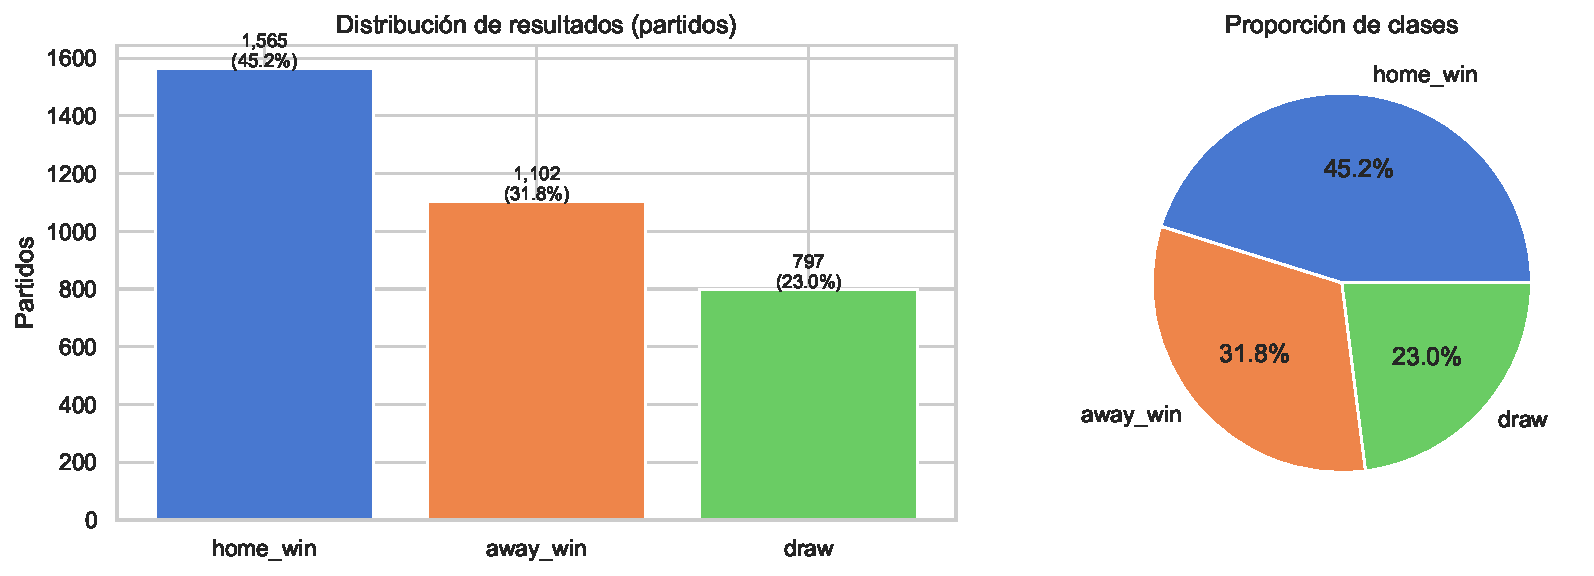
\includegraphics[width=0.85\textwidth]{assets/figuras/eda/balance_clases.pdf}
    \caption{Distribución de la variable objetivo en el dataset}
    \label{fig:balance_clases}
\end{figure}

El desequilibrio tiene dos implicaciones directas para el modelado. Un clasificador que predijera siempre \texttt{home\_win} obtendría una precisión del 45,2\% sin aprender ningún patrón, por lo que el \textit{accuracy} por sí solo no es una métrica válida y se usarán F1-score macro y ponderado en su lugar. Además, se aplicará \texttt{class\_weight='balanced'} en los clasificadores que lo soporten para penalizar más los errores en las clases minoritarias.

El análisis por separado de las competiciones femeninas y masculinas muestra diferencias relevantes. En las masculinas (2.924 partidos) la distribución es 44,8\% victorias locales, 31,0\% visitantes y 24,2\% empates. En las femeninas (540 partidos) los empates caen al 16,7\% y las victorias visitantes suben al 36,1\%. Esta diferencia justifica incluir una variable binaria que identifique el tipo de competición en el dataset de modelado.

\begin{figure}[H]
    \centering
    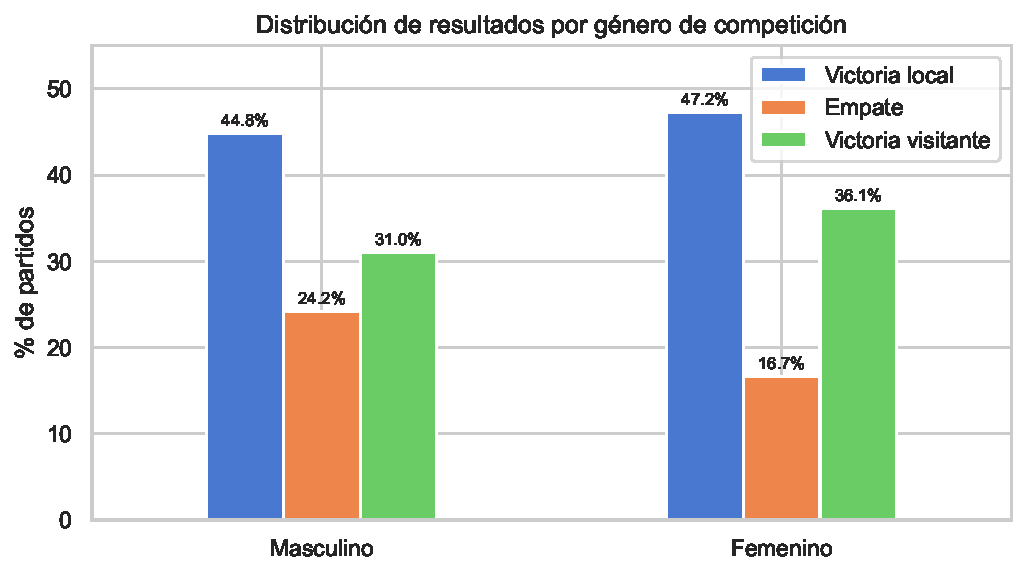
\includegraphics[width=0.80\textwidth]{assets/figuras/eda/balance_genero.pdf}
    \caption{Distribución de resultados por género de competición}
    \label{fig:balance_genero}
\end{figure}

\subsubsection{Análisis temporal}

El modelo predice el resultado a partir del estado acumulado del partido hasta un minuto determinado. Antes de construir ese dataset de modelado, conviene verificar que los datos registran la evolución del partido de forma homogénea y decidir cómo tratar los eventos que quedan fuera de los 90 minutos reglamentarios.

Al observar la distribución del minuto de cada evento se aprecia un comportamiento que encaja con lo que ocurre en un partido real. Los picos de actividad se producen al inicio de cada parte, en los minutos 1 y 46, cuando se realizan los saques de centro, y a partir de ahí la densidad de eventos se mantiene estable hasta el final del tiempo reglamentario. No hay ningún periodo del partido con un volumen de eventos anómalamente bajo o alto.

Lo que sí requiere una decisión explícita es qué hacer con los eventos registrados pasado el minuto 90. El dataset incluye partidos con prórroga, ya que el minuto máximo registrado es el 139, y prácticamente todos los partidos tienen al menos algún evento fuera de los 90 minutos reglamentarios. Dado que el tiempo de descuento varía según las interrupciones de cada partido y la prórroga no tiene duración fija, mantener esos eventos complicaría la construcción del dataset sin aportar una mejora clara. Por ello se opta por truncar al minuto 90, lo que afecta al 3,2\% de los eventos y deja una base temporal homogénea para todos los partidos.

Respecto a los goles, la segunda parte acumula algo más de la mitad del total, 4.978 de 9.150, frente a los 4.172 de la primera. El minuto 47, el primero tras el descanso, es el de mayor densidad de goles de todo el dataset. Este comportamiento confirma que el momento del partido en el que se está haciendo la predicción aporta información relevante al modelo. La tabla~\ref{tab:temporal} recoge los principales indicadores del análisis.

\begin{table}[H]
    \centering
    \begin{tabular}{lr}
        \hline
        \textbf{Indicador}                                     & \textbf{Valor} \\
        \hline
        Eventos en tiempo reglamentario ($\leq 90$ min)        & 96,8\%         \\
        Eventos en tiempo de descuento / prórroga ($> 90$ min) & 3,2\%          \\
        Partidos con algún evento en minuto $> 90$             & 3.354 de 3.464 \\
        Minuto máximo registrado                               & 139            \\
        \hline
        Goles en primera parte (min.\ 1--45)                   & 4.172 (45,6\%) \\
        Goles en segunda parte (min.\ 46--90)                  & 4.978 (54,4\%) \\
        Minuto con más goles                                   & 47 (143 goles) \\
        \hline
    \end{tabular}
    \caption{Principales indicadores del análisis temporal}
    \label{tab:temporal}
\end{table}

\subsubsection{xG y features discriminativas}

Para decidir qué variables incluir en el modelo, se ha analizado cuáles de las métricas del partido guardan mayor relación con el resultado. El método utilizado consiste en calcular, para cada partido, la diferencia entre el valor acumulado del equipo local y el del visitante en cada métrica, y medir cuánto se correlaciona esa diferencia con haber ganado o perdido.

El xG es la métrica que mejor separa los resultados, con una correlación de $r = 0{,}568$ entre la diferencia de xG y el resultado del partido. Le siguen los tiros ($r = 0{,}357$) y los pases ($r = 0{,}289$). En los tres casos el patrón es claro, ya que el equipo que acaba ganando acumula más xG, más tiros y más pases que el que pierde. La figura~\ref{fig:correlacion_features} muestra el valor de correlación para cada métrica.

Las presiones y las faltas van en sentido contrario. La diferencia entre el local y el visitante correlaciona negativamente con el resultado ($r = -0{,}223$ y $r = -0{,}199$), lo que significa que el equipo local presiona más y comete más faltas en los partidos que pierde. La explicación es táctica, ya que el equipo que va perdiendo aumenta su intensidad defensiva para intentar recuperar el balón, lo que se traduce en más presiones y más faltas. Estas métricas son útiles para el modelo, pero hay que tener en cuenta que el equipo que más presiona no es el que va ganando, sino el que va perdiendo.

\begin{figure}[H]
    \centering
    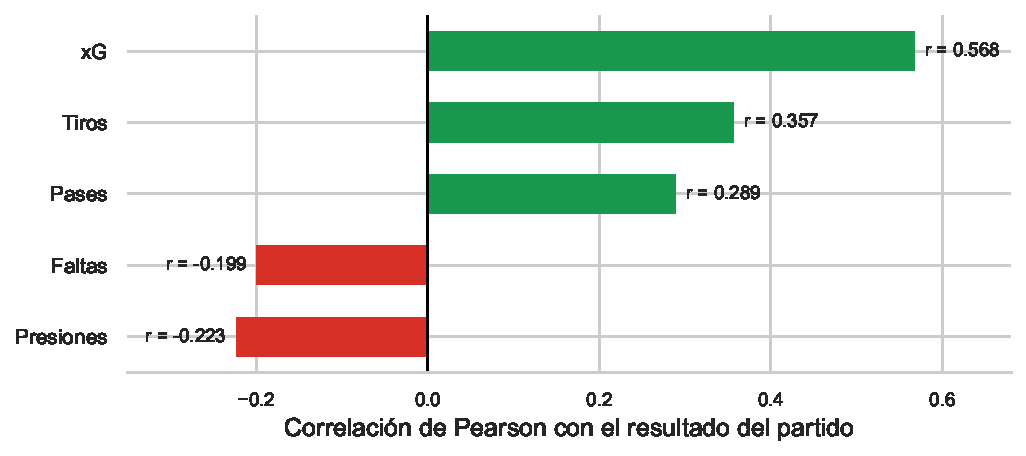
\includegraphics[width=0.82\textwidth]{assets/figuras/eda/correlacion_features.pdf}
    \caption{Correlación de Pearson entre la diferencia de cada métrica acumulada y el resultado del partido}
    \label{fig:correlacion_features}
\end{figure}

La tasa de pases completados también varía según el resultado. El equipo ganador completa alrededor de cuatro puntos porcentuales más de sus pases que el perdedor, tanto cuando gana el local (78,6\% frente a 74,0\%) como cuando gana el visitante (77,4\% frente a 74,3\%). Completar más pases es un indicador de control del partido, y el dato confirma que esta métrica aporta información útil al modelo.

Finalmente, conviene remarcar que el 35,3\% de los partidos se decide por un solo gol, lo que hace que muchos encuentros sean difíciles de predecir hasta el final. Además, 231 partidos terminan 0-0, y en esos casos el modelo no dispone de diferencial de goles ni de xG relevante, por lo que tendrá que apoyarse en métricas de posesión y control como los pases, las presiones o los duelos.

\subsubsection{Marcador en curso}

Entre todas las variables que se pueden construir a partir del dataset, el marcador en el minuto $t$ es la más predictiva para un modelo de probabilidad de victoria. Si un equipo gana por dos goles en el minuto 80, la probabilidad de que mantenga el resultado es muy alta independientemente de cualquier otra métrica. Sin embargo, el marcador en curso no existe como campo en el dataset, ya que los datos de StatsBomb registran eventos individuales, no el estado acumulado del partido.

El marcador puede derivarse acumulando los eventos de tipo \textit{Shot} cuyo \texttt{shot\_outcome} sea \texttt{Goal}, ordenados por minuto. Para cada minuto del partido se cuenta cuántos goles ha marcado cada equipo hasta ese momento, lo que produce una curva escalonada que refleja la evolución del marcador a lo largo del encuentro. La figura~\ref{fig:marcador_en_curso} muestra esta evolución para un partido de ejemplo, junto con la diferencia de goles en cada minuto.

\begin{figure}[H]
    \centering
    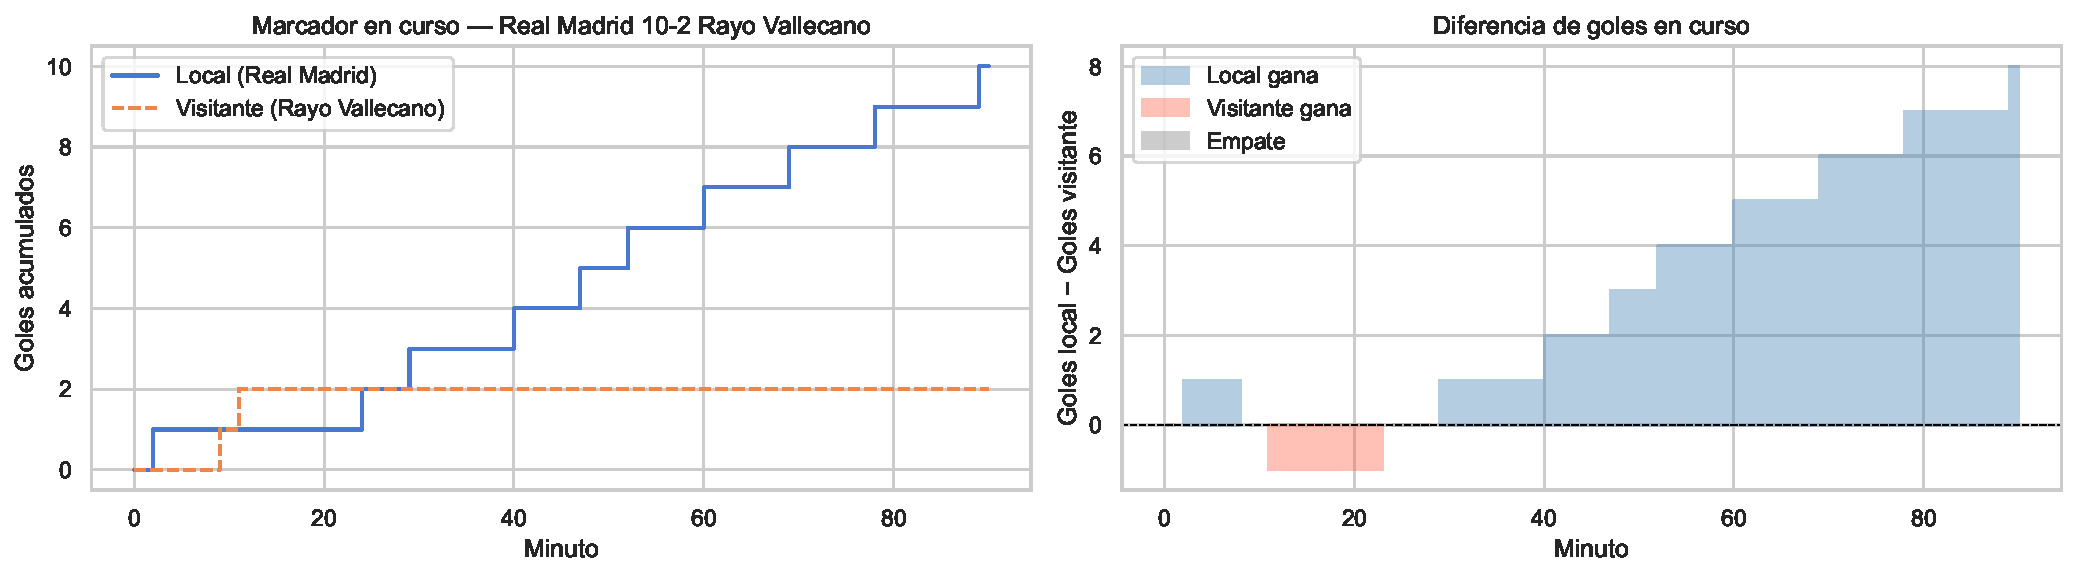
\includegraphics[width=0.95\textwidth]{assets/figuras/eda/marcador_en_curso.pdf}
    \caption{Evolución del marcador en curso y diferencia de goles para un partido de ejemplo}
    \label{fig:marcador_en_curso}
\end{figure}

Este análisis confirma que la derivación es viable para todos los partidos del dataset y que los goles están correctamente registrados como eventos \textit{Shot} con resultado \texttt{Goal}. El marcador en curso será una de las variables construidas en la fase de preparación de datos.

\subsubsection{Calidad de los datos}

El análisis de valores ausentes refleja una estructura dispersa habitual en datasets de eventos deportivos, donde cada columna solo tiene valores para el subconjunto de filas correspondiente a su tipo de evento. La columna \texttt{xg} presenta un 99,28\% de nulos porque únicamente se registra en tiros; \texttt{pass\_length} y \texttt{pass\_angle} tienen un 72,21\% de nulos al aplicar solo a pases; y \texttt{card\_type} alcanza el 99,88\% al estar reservada para tarjetas. Todos estos nulos son estructuralmente esperables y no representan un problema de calidad.

Los campos clave para el modelado no presentan ningún valor ausente, lo que confirma la integridad del dataset. Entre ellos se encuentran \texttt{match\_id}, \texttt{minute}, \texttt{event\_type}, \texttt{is\_home} y \texttt{final\_result}. Las columnas de localización (\texttt{loc\_x}, \texttt{loc\_y}) muestran un 0,75\% de nulos, correspondientes a eventos administrativos como el inicio de periodo, que no tienen posición en el campo asociada.

\subsubsection{Limitaciones del dataset}

El análisis exploratorio ha permitido identificar las principales limitaciones del dataset, algunas de las cuales ya se han comentado en apartados anteriores junto con las decisiones adoptadas para mitigarlas.

La limitación más relevante que no se ha abordado todavía es el sesgo hacia el fútbol de élite. Todos los partidos del dataset pertenecen a competiciones profesionales de alto nivel, principalmente ligas europeas y torneos internacionales. La Liga española es la más representada, con 868 partidos (el 25,1\% del total), lo que introduce cierta concentración geográfica. Los patrones aprendidos por el modelo pueden no generalizarse bien a ligas de niveles inferiores o con estilos de juego muy distintos. Para el objetivo de este trabajo esto no supone un problema, pero es un factor a tener en cuenta si se quisiera aplicar el modelo fuera del contexto de las competiciones incluidas.

Las demás limitaciones ya han sido tratadas a lo largo del análisis. La diferencia entre el fútbol femenino y masculino se aborda incluyendo una variable binaria en el dataset de modelado (apartado de balance de clases). La ausencia del marcador en tiempo real se resuelve derivándolo a partir de los eventos de tipo \textit{Shot} con resultado \texttt{Goal} (apartado de marcador en curso). El truncado al minuto 90 elimina el 3,2\% de los eventos y deja fuera los partidos con prórroga, lo que introduce cierto ruido en la variable objetivo para ese subconjunto (apartado de análisis temporal). Por último, la estructura dispersa del dataset requiere una transformación en métricas acumuladas antes del modelado, tal y como se describe en el apartado de calidad de los datos.

\subsection{Preparación del dataset de modelado}

El objetivo de esta fase es transformar el dataset de eventos obtenido en el apartado anterior en un conjunto de datos directamente utilizable por los algoritmos de aprendizaje automático. El dataset original contiene una fila por cada acción registrada en los partidos, por lo que debemos convertirlo a un formato que permita representar el estado de cada partido en un minuto determinado. Para ello, se genera una fila por cada par \textit{(partido, minuto)}, de modo que para cada uno de los 3.464 partidos del dataset se generan noventa filas, una por cada minuto del tiempo reglamentario.  La granularidad de un minuto nos permite determinar con mayor precisión a partir de qué instantes del partido el modelo es capaz de predecir el resultado del encuentro, y permite agregar los valores para construir variables de ventana deslizante. El resultado es un dataset de 311.760 registros y 48 variables de entrada.

\subsubsection{Tratamiento del tiempo reglamentario y el tiempo de descuento}

Como se ha visto en el capítulo anterior, el dataset de eventos incluye acciones correspondientes al tiempo reglamentario, al tiempo de descuento y, en los partidos con prórroga, a los periodos adicionales. Para la construcción del dataset de modelado se adoptan las siguientes decisiones:

\begin{itemize}
    \item \textbf{Prórroga y penaltis (periodos 3 a 5):} se excluyen de las variables de entrada. La duración de la prórroga no es fija entre partidos ni entre competiciones, y su estructura difiere del tiempo reglamentario, lo que exigiría un tratamiento diferenciado que añadiría complejidad sin beneficio claro para el objetivo del trabajo. La variable objetivo (\texttt{final\_result}) sí refleja el resultado definitivo del partido, incluido el desenlace en prórroga o penaltis cuando corresponda, de modo que la información sobre el resultado final se preserva íntegramente.

    \item \textbf{Tiempo de descuento (minuto $> 90$, periodo 2):} los eventos registrados en tiempo de descuento representan el 3,2\% del total, tal como se constató en el análisis exploratorio. Dado que el tiempo de descuento varía en función de las interrupciones de cada partido y no tiene una duración homogénea entre encuentros, estos eventos se reasignan al \textit{snapshot} del minuto 90, integrándolos en el estado acumulado de ese minuto. Esta decisión garantiza que cualquier gol marcado en el descuento quede recogido en el estado final del partido sin necesidad de modelar minutos variables más allá de los 90 reglamentarios.
\end{itemize}

\subsubsection{Indicadores de actividad y estado acumulado}

A partir del dataset filtrado se definen 15 indicadores binarios y la variable de \textit{expected goals} (\textit{xG}). Cada tipo de evento del dataset se convierte en un vector binario, de modo que podamos representar el total de acciones de esa clase realizadas por un equipo desde el inicio del partido hasta un minuto $t$.

Los indicadores definidos son: gol, tiro, tiro a puerta, tiro en el área, pase, pase completado, presión defensiva, duelo ganado, despeje, bloqueo, conducción de balón, tarjeta amarilla, tarjeta roja, y entrada en el tercio de ataque. El \textit{xG} se trata como variable continua y toma el valor 0 para todos los eventos que no corresponden a un tiro.

El estado acumulado de las variables se calcula aplicando una suma acumulativa sobre los eventos ordenados por minuto dentro de cada grupo \textit{(partido, equipo)}. Para rellenar los minutos en los que no se registra ningún evento, se usarán los valores anteriores mediante propagación hacia adelante (\textit{forward fill}), lo que equivale a mantener el estado del partido sin cambios hasta que se produzca una nueva acción. Los minutos anteriores al primer evento del partido se inicializan a cero.

\subsubsection{Variables de ventana deslizante}

Las variables acumuladas desde el inicio del partido capturan el estado global del encuentro, pero no distinguen si una acción tuvo lugar en el minuto 5 o en el 85. Para medir la intensidad de juego reciente e incorporar una dimensión de \textit{momentum}, se calculan tres variables de ventana deslizante de 15 minutos: el \textit{xG} generado en los últimos 15 minutos (\texttt{xg\_last15}), el número de tiros en ese mismo intervalo (\texttt{shots\_last15}) y el número de presiones defensivas (\texttt{pressures\_last15}). Estas variables se obtienen eficientemente como la diferencia entre el valor acumulado en el minuto $t$ y el valor acumulado en el minuto $t - 15$, que se extrae desplazando la serie temporal 15 posiciones hacia adelante dentro de cada grupo \textit{(partido, equipo)}.

La selección de \textit{xG}, tiros y presiones para las variables de ventana responde a los resultados del análisis exploratorio, donde estas métricas presentaron las mayores correlaciones con el resultado final. Extender la ventana al conjunto completo de indicadores añadiría 30 variables con un coste computacional significativo y una contribución marginal previsiblemente reducida, dado que las tres seleccionadas cubren las dimensiones ofensiva (\textit{xG} y tiros) y defensiva (presiones) del juego reciente.

\subsubsection{Variables derivadas y \textit{feature engineering}}

Una vez disponibles las estadísticas acumuladas y las variables de ventana para ambos equipos, se construye la representación definitiva del estado del partido, representando ambos equipos en una única fila por \textit{(partido, minuto)}, duplicando las columnas y añadiendo sufijos \texttt{\_home} y \texttt{\_away} que permitan representar el equipo al que corresponden. Además, se generan unas variables o \textit{features} que, aunque no aportan nueva información, permiten transformar la semántica de las variables y su efecto en la calibración de los modelos. Las variables derivadas construidas son las siguientes:

\begin{itemize}
    \item \textbf{Diferenciales del marcador} (\texttt{score\_diff}, \texttt{xg\_diff}, \texttt{shots\_diff}): diferencia entre el valor del equipo local y el del visitante para los goles, el \textit{xG} acumulado y el número de tiros. Sintetizan en un único valor la ventaja o desventaja relativa de cada equipo en cada dimensión, evitando que el modelo tenga que aprender implícitamente esta operación de resta.

    \item \textbf{Posesión del balón} (\texttt{possession\_home}): proporción de conducciones de balón realizadas por el equipo local sobre el total de conducciones del partido. StatsBomb no proporciona una métrica directa de posesión, y las conducciones (\textit{carries}), que registran el desplazamiento físico del balón por parte de un jugador, constituyen la aproximación más precisa disponible en el dataset. En los minutos previos al primer evento registrado se asigna un valor de 0,5 como posesión neutra.

    \item \textbf{Tasa de pase completado} (\texttt{pass\_completion\_home}, \texttt{pass\_completion\_away}): cociente entre los pases completados y los pases intentados para cada equipo. Captura la calidad y el control en la circulación del balón, que el análisis exploratorio confirmó que correlaciona positivamente con la victoria, con una diferencia de aproximadamente cuatro puntos porcentuales entre equipos ganadores y perdedores.

    \item \textbf{Total de goles} (\texttt{total\_goals}): suma de los goles marcados por ambos equipos hasta el minuto $t$. Un partido con marcador 3-3 presenta un perfil dinámico muy distinto a uno con 0-0, aun cuando \texttt{score\_diff} sea cero en ambos casos. Esta variable permite al modelo distinguir entre partidos abiertos, con muchos goles y mayor probabilidad de nuevas anotaciones, y partidos cerrados de carácter más defensivo.

    \item \textbf{Calidad ofensiva por tiro} (\texttt{xg\_per\_shot\_home}, \texttt{xg\_per\_shot\_away}): cociente entre el \textit{xG} acumulado y el número de tiros realizados. Diferencia entre equipos que generan ocasiones de alta peligrosidad, principalmente desde dentro del área, y aquellos con un volumen elevado de tiros de escasa probabilidad de gol. En los minutos anteriores al primer tiro del equipo se asigna el valor cero.

    \item \textbf{Sobrerendimiento respecto al xG} (\texttt{goals\_minus\_xg\_home}, \texttt{goals\_minus\_xg\_away}): diferencia entre los goles marcados y el \textit{xG} acumulado. Un valor positivo indica que el equipo está materializando más goles de los que cabría esperar a partir de la calidad de sus ocasiones, lo que puede responder tanto a una finalización de alta efectividad como a factores de varianza aleatoria. Un valor negativo refleja la situación contraria, señalando que el equipo está creando peligro sin traducirlo en goles.

    \item \textbf{Tipo de competición} (\texttt{is\_womens}): indicador binario que distingue las competiciones femeninas de las masculinas. El análisis exploratorio reveló diferencias sistemáticas en la distribución de resultados entre ambos contextos: los empates representan el 16,7\,\% de los partidos femeninos frente al 24,2\,\% en los masculinos, y las victorias visitantes alcanzan el 36,1\,\% en el fútbol femenino frente al 31,0\,\% en el masculino. Estas diferencias justifican incluir esta variable para que el modelo pueda calibrar sus probabilidades en función del tipo de competición.
\end{itemize}

\subsubsection{Composición final del dataset de modelado}

El dataset resultante contiene 311.760 filas, correspondientes a los 3.464 partidos del conjunto de datos y sus 90 minutos reglamentarios, y 48 variables de entrada agrupadas en ocho categorías. La tabla~\ref{tab:features} resume la composición del dataset. La integridad del conjunto fue verificada mediante tres comprobaciones: ausencia de valores ausentes en las columnas clave para el modelado, coincidencia entre el marcador derivado y el marcador real de un partido de muestra seleccionado aleatoriamente, y correspondencia exacta entre el número de filas generadas y el producto del número de partidos por el número de minutos.

\begin{table}[H]
    \centering
    \begin{tabular}{lcp{7.5cm}}
        \hline
        \textbf{Categoría}           & \textbf{Variables} & \textbf{Descripción}                                                                                                                                                                                                                                     \\
        \hline
        Estadísticas acumuladas      & 28                 & Goles, tiros, tiros a puerta, tiros en el área, pases, presiones, duelos ganados, despejes, bloqueos, conducciones, tarjetas amarillas, tarjetas rojas, entradas en el tercio de ataque y \textit{xG}; para el equipo local y el visitante por separado. \\[4pt]
        Ventana deslizante (15\,min) & 6                  & \textit{xG}, tiros y presiones en los últimos 15 minutos; para el equipo local y el visitante.                                                                                                                                                           \\[4pt]
        Diferenciales                & 3                  & Diferencia local-visitante de goles (\texttt{score\_diff}), \textit{xG} (\texttt{xg\_diff}) y tiros (\texttt{shots\_diff}).                                                                                                                              \\[4pt]
        Control y posesión           & 4                  & Posesión del local, tasa de pase completado de ambos equipos y total de goles.                                                                                                                                                                           \\[4pt]
        Calidad ofensiva             & 4                  & \textit{xG} por tiro y sobrerendimiento respecto al \textit{xG}; para ambos equipos.                                                                                                                                                                     \\[4pt]
        Superioridad numérica        & 1                  & Diferencial de jugadores en campo (\texttt{players\_diff}).                                                                                                                                                                                              \\[4pt]
        Tiempo restante              & 1                  & Minutos restantes hasta el final del tiempo reglamentario.                                                                                                                                                                                               \\[4pt]
        Tipo de competición          & 1                  & Indicador binario de competición femenina (\texttt{is\_womens}).                                                                                                                                                                                         \\
        \hline
        \textbf{Total}               & \textbf{48}        &                                                                                                                                                                                                                                                          \\
        \hline
        \multicolumn{3}{l}{\small Fuente: elaboración propia.}
    \end{tabular}
    \caption{Categorías de variables del dataset de modelado}
    \label{tab:features}
\end{table}
\section{Modelado y comparativa}

\subsection{Planteamiento de la comparativa}

Los modelos se evalúan sobre el conjunto de test formado por las temporadas 2020-2025, con 692 partidos y 62.280 filas. Las tres métricas principales son el \textit{accuracy} global, el F1-score macro y la pérdida logarítmica (\textit{log-loss}). El F1-score macro promedia el F1 de las tres clases con el mismo peso, lo que penaliza por igual los errores en las clases minoritarias. La pérdida logarítmica evalúa la calidad de las probabilidades predichas, no solo la clase asignada.

Adicionalmente, se calcula el \textit{accuracy} en seis instantes del partido: los minutos 15, 30, 45, 60, 75 y 90. Este análisis temporal permite cuantificar a partir de qué momento el modelo supera el umbral de referencia del 70\,\% y cómo evoluciona la confianza de la predicción conforme avanza el encuentro.

La línea base del problema es predecir siempre la clase mayoritaria (victoria local), con un 45,2\,\% de \textit{accuracy}. Cualquier modelo útil debe superar este valor de forma sustancial.

\subsection{Modelos seleccionados}

Se entrenan y comparan tres clasificadores: Random Forest, XGBoost y SVM lineal.

\textbf{Random Forest} construye un conjunto de árboles de decisión sobre submuestras aleatorias del dataset y combina sus predicciones por votación mayoritaria. No requiere normalización de variables, gestiona bien las interacciones entre variables sin configuración adicional y permite interpretar el modelo mediante la importancia de cada variable. Se utiliza como modelo de referencia.

\textbf{XGBoost} es un método de potenciación del gradiente que construye los árboles de forma secuencial. Cada árbol corrige los errores del árbol anterior minimizando una función de pérdida regularizada. En clasificación sobre datos tabulares estructurados, este método suele superar al Random Forest gracias a su mayor capacidad de ajuste y a la regularización incorporada. Es el modelo principal del trabajo.

El \textbf{SVM lineal} se incluye como un tercer modelo de comparación. Este tipo de modelo busca separar las clases mediante márgenes de decisión, por lo que puede resultar útil para comprobar si el problema puede resolverse adecuadamente con una frontera de decisión más simple. En este trabajo se utiliza una versión lineal del SVM, ya que el dataset contiene un número elevado de filas y un SVM con kernel no lineal tendría un coste computacional mucho mayor. A diferencia de Random Forest y XGBoost, este modelo sí requiere normalizar las variables de entrada antes del entrenamiento.


Se consideró también el uso de una red neuronal recurrente (LSTM) para aprovechar la naturaleza secuencial de las series minuto a minuto, pero fue descartada por la complejidad adicional de diseño y validación que implicaría.

\subsection{Ajuste de hiperparámetros}

El Random Forest se configura con 300 árboles y pesos de clase balanceados (\texttt{class\_weight='balanced'}), que asignan mayor penalización a los errores en las clases minoritarias. No se realiza búsqueda sistemática de hiperparámetros para este modelo, que actúa como referencia estable.

XGBoost se configura con 300 estimadores, profundidad máxima 6, tasa de aprendizaje 0,1 y tasas de submuestreo de 0,8 por fila y por columna. El desequilibrio de clases se gestiona asignando a cada muestra de entrenamiento un peso inversamente proporcional a la frecuencia de su clase, calculado con la estrategia \texttt{balanced} de scikit-learn. Al igual que con el Random Forest, no se realiza una búsqueda sistemática de hiperparámetros en esta fase.

Para el SVM se utiliza un flujo ligeramente distinto, ya que este modelo es sensible a la escala de las variables y no proporciona probabilidades directamente. En primer lugar, las variables de entrada se normalizan mediante \texttt{StandardScaler}. Después, se evalúan distintos valores del parámetro \texttt{C}, que controla el equilibrio entre margen amplio y penalización de errores de clasificación. Los valores probados son 0,01, 0,1, 1, 10 y 100, seleccionando el mejor valor según el F1-score macro en una partición interna de validación.

La división interna utilizada para el SVM se realiza únicamente dentro del conjunto de entrenamiento, manteniendo intacto el conjunto de test empleado por el resto de modelos. Esta división separa los datos en tres subconjuntos: uno para ajustar el modelo, otro para seleccionar el valor de \texttt{C} y otro para calibrar las probabilidades. La calibración se realiza porque \texttt{LinearSVC} no genera probabilidades de forma directa, pero estas son necesarias para calcular la pérdida logarítmica y comparar el modelo con Random Forest y XGBoost bajo las mismas métricas.

\subsection{Resultados comparativos}

\subsubsection{Random Forest}

El Random Forest obtiene un \textit{accuracy} global del 66,0\,\%, un F1-score macro del 59,2\,\% y una pérdida logarítmica de 0,769 sobre el conjunto de test. La tabla~\ref{tab:resultados_rf} recoge el \textit{accuracy} y el F1-score macro para los seis puntos de corte evaluados.

\begin{table}[H]
    \centering
    \begin{tabular}{rcc}
        \hline
        \textbf{Minuto} & \textbf{Accuracy} & \textbf{Macro-F1} \\
        \hline
        15              & 55,6\%            & 44,4\%            \\
        30              & 60,0\%            & 48,0\%            \\
        45              & 64,2\%            & 54,4\%            \\
        60              & 71,0\%            & 64,9\%            \\
        75              & 76,7\%            & 73,3\%            \\
        90              & 91,3\%            & 90,4\%            \\
        \hline
        \multicolumn{3}{l}{\small Fuente: elaboración propia.}
    \end{tabular}
    \caption{\textit{Accuracy} y Macro-F1 del Random Forest por minuto de partido}
    \label{tab:resultados_rf}
\end{table}

El modelo supera el 70\,\% de \textit{accuracy} en el minuto 60. Con la mitad del partido disputado, el modelo predice correctamente el resultado final en siete de cada diez partidos. La figura~\ref{fig:accuracy_rf} muestra la evolución por minuto y la figura~\ref{fig:confusion_rf} la matriz de confusión normalizada.

\begin{figure}[H]
    \centering
    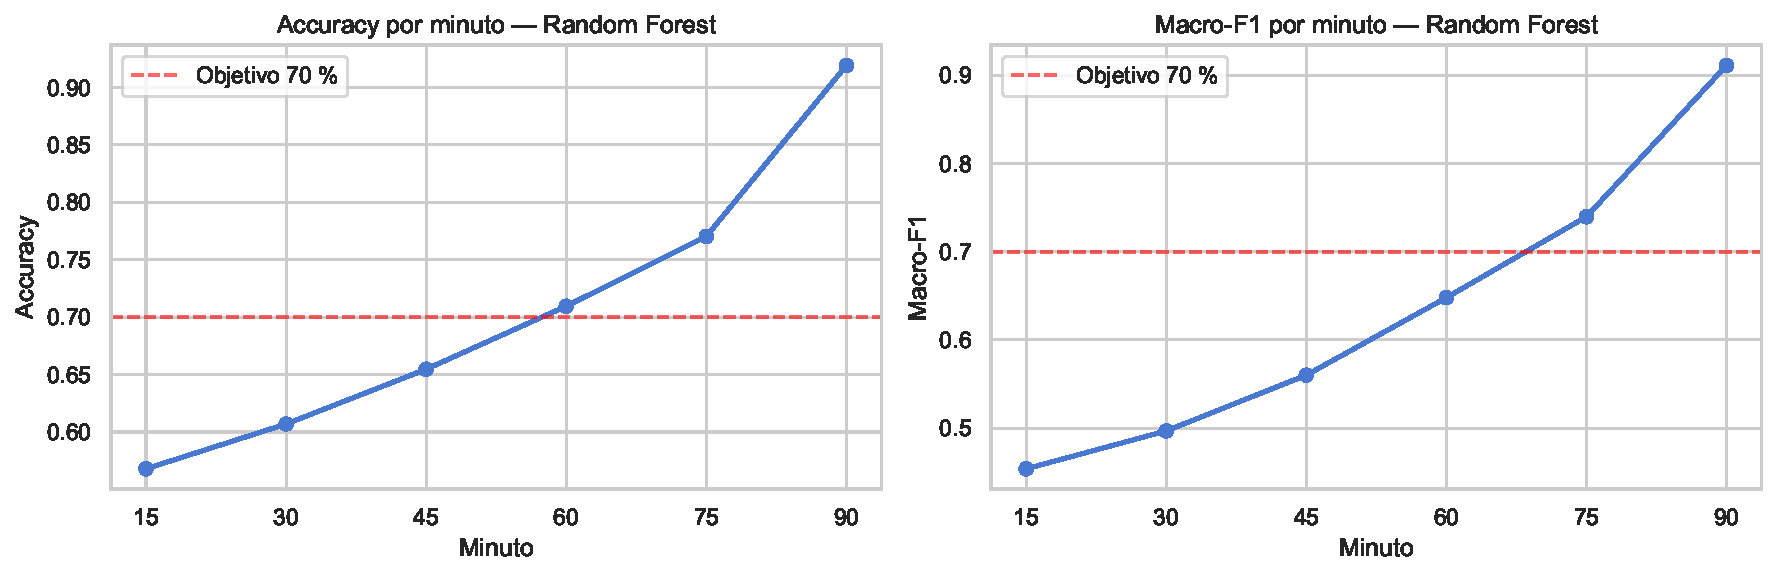
\includegraphics[width=0.90\textwidth]{assets/figuras/modeling/accuracy_por_minuto_rf.pdf}
    \caption{Evolución del \textit{accuracy} y el Macro-F1 por minuto de partido para el Random Forest}
    \label{fig:accuracy_rf}
\end{figure}

\begin{figure}[H]
    \centering
    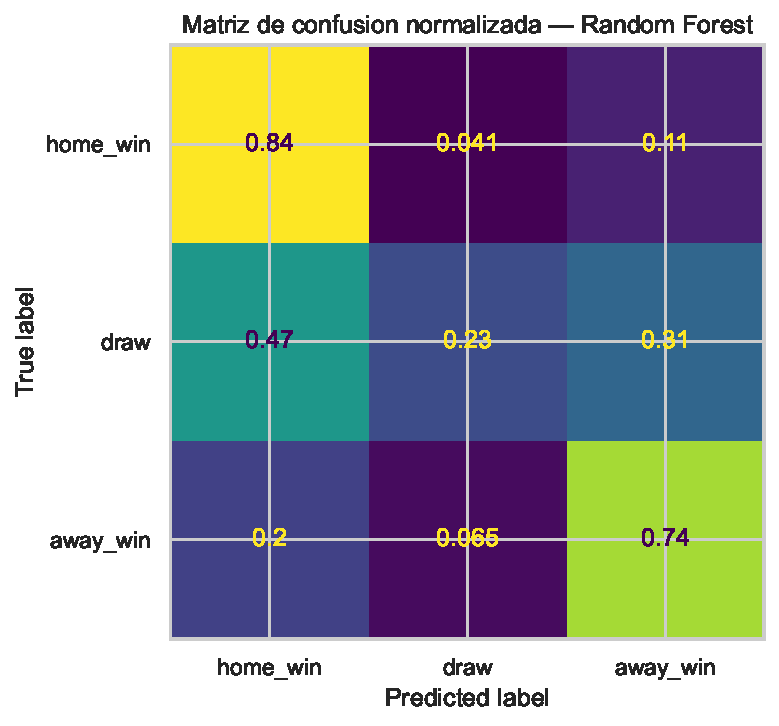
\includegraphics[width=0.55\textwidth]{assets/figuras/modeling/confusion_rf.pdf}
    \caption{Matriz de confusión normalizada del Random Forest sobre el conjunto de test}
    \label{fig:confusion_rf}
\end{figure}

La clase con menor rendimiento es el empate, con un F1 del 33\,\%, frente al 75\,\% de la victoria local y el 70\,\% de la victoria visitante. El empate es difícil de anticipar, ya que pequeñas variaciones en los últimos minutos pueden convertirlo en victoria para cualquiera de los dos equipos. El análisis de importancia de variables (figura~\ref{fig:importancia_rf}) confirma que \texttt{score\_diff}, el \textit{xG} acumulado y \texttt{minutes\_remaining} son las variables más determinantes, junto con las métricas de tiro recientes.

\begin{figure}[H]
    \centering
    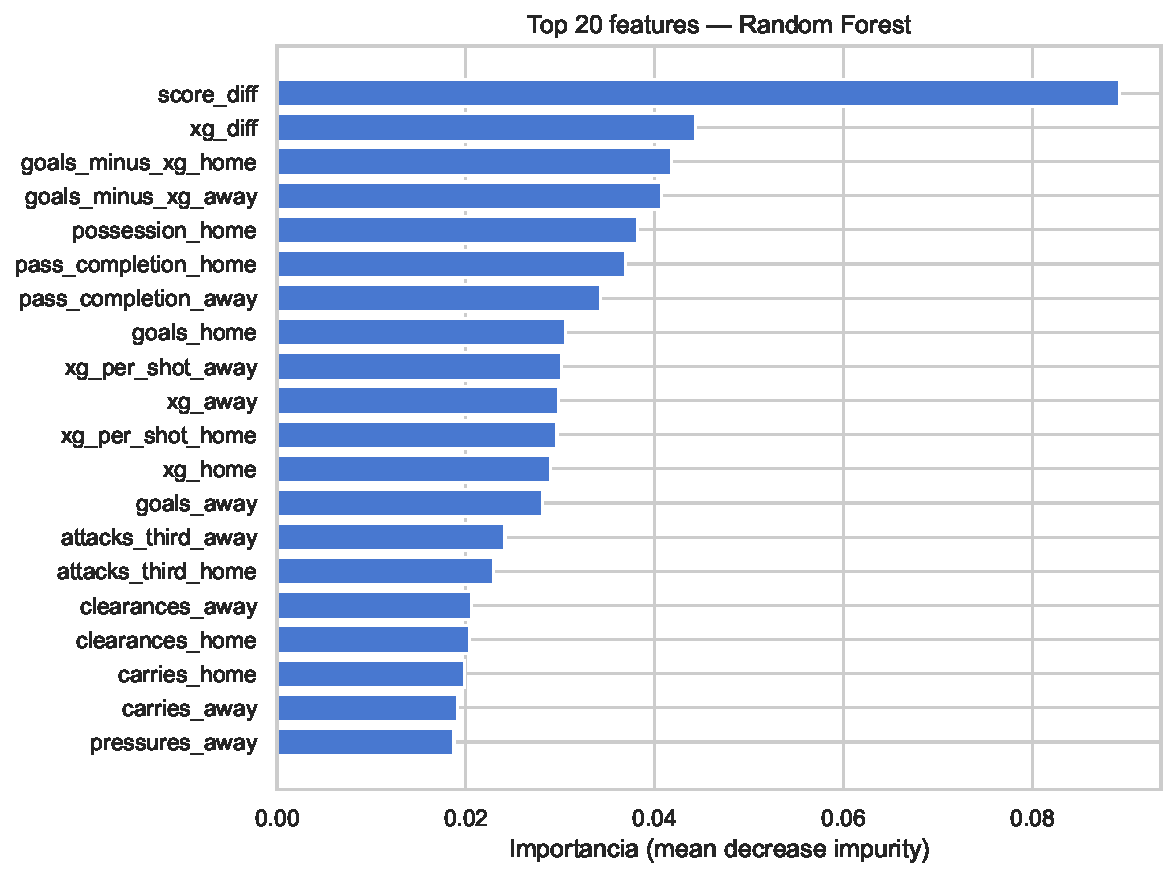
\includegraphics[width=0.80\textwidth]{assets/figuras/modeling/feature_importance_rf.pdf}
    \caption{Importancia de las 20 variables más relevantes en el Random Forest}
    \label{fig:importancia_rf}
\end{figure}

\subsubsection{XGBoost}

El XGBoost obtiene un \textit{accuracy} global del 64,8\,\%, un F1-score macro del 61,3\,\% y una pérdida logarítmica de 0,774 sobre el conjunto de test. La tabla~\ref{tab:resultados_xgb} recoge el \textit{accuracy} y el F1-score macro por minuto.

\begin{table}[H]
    \centering
    \begin{tabular}{rcc}
        \hline
        \textbf{Minuto} & \textbf{Accuracy} & \textbf{Macro-F1} \\
        \hline
        15              & 53,3\%            & 48,8\%            \\
        30              & 60,3\%            & 55,9\%            \\
        45              & 62,6\%            & 58,2\%            \\
        60              & 69,5\%            & 66,2\%            \\
        75              & 76,4\%            & 74,0\%            \\
        90              & 90,6\%            & 89,7\%            \\
        \hline
        \multicolumn{3}{l}{\small Fuente: elaboración propia.}
    \end{tabular}
    \caption{\textit{Accuracy} y Macro-F1 del XGBoost por minuto de partido}
    \label{tab:resultados_xgb}
\end{table}

El modelo alcanza el 69,5\,\% de \textit{accuracy} en el minuto 60, ligeramente por debajo del umbral del 70\,\%. La figura~\ref{fig:accuracy_xgb} muestra la evolución temporal y la figura~\ref{fig:confusion_xgb} la matriz de confusión normalizada.

\begin{figure}[H]
    \centering
    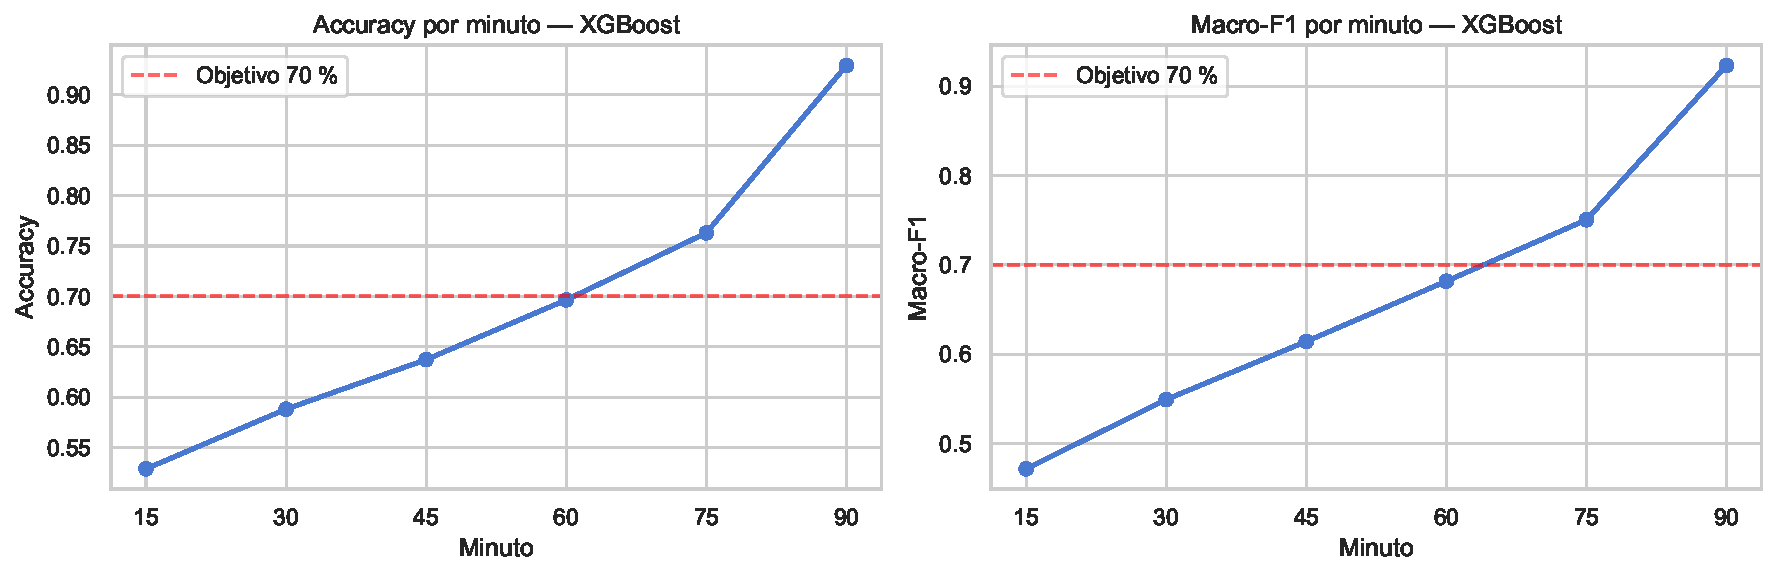
\includegraphics[width=0.90\textwidth]{assets/figuras/modeling/accuracy_por_minuto_xgb.pdf}
    \caption{Evolución del \textit{accuracy} y el Macro-F1 por minuto de partido para el XGBoost}
    \label{fig:accuracy_xgb}
\end{figure}

\begin{figure}[H]
    \centering
    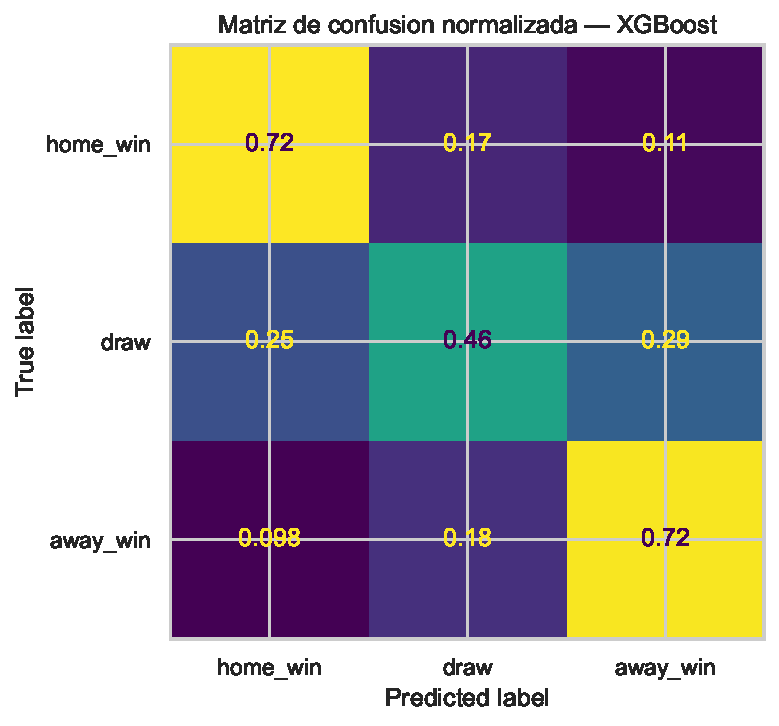
\includegraphics[width=0.55\textwidth]{assets/figuras/modeling/confusion_xgb.pdf}
    \caption{Matriz de confusión normalizada del XGBoost sobre el conjunto de test}
    \label{fig:confusion_xgb}
\end{figure}

La diferencia más destacada respecto al Random Forest es el rendimiento en la clase del empate: el XGBoost obtiene un F1 del 42\,\% frente al 33\,\% del Random Forest, lo que refleja que los pesos de muestra balanceados aplicados durante el entrenamiento consiguen mejorar la detección de la clase minoritaria. Esta mejora en el empate eleva el F1-score macro (61,3\,\% frente a 59,2\,\%), pero se produce a costa de un ligero descenso en el \textit{accuracy} global (64,8\,\% frente a 66,0\,\%). El análisis de importancia de variables (figura~\ref{fig:importancia_xgb}) refleja un patrón similar al del Random Forest, con \texttt{score\_diff} y el \textit{xG} como variables dominantes.

\begin{figure}[H]
    \centering
    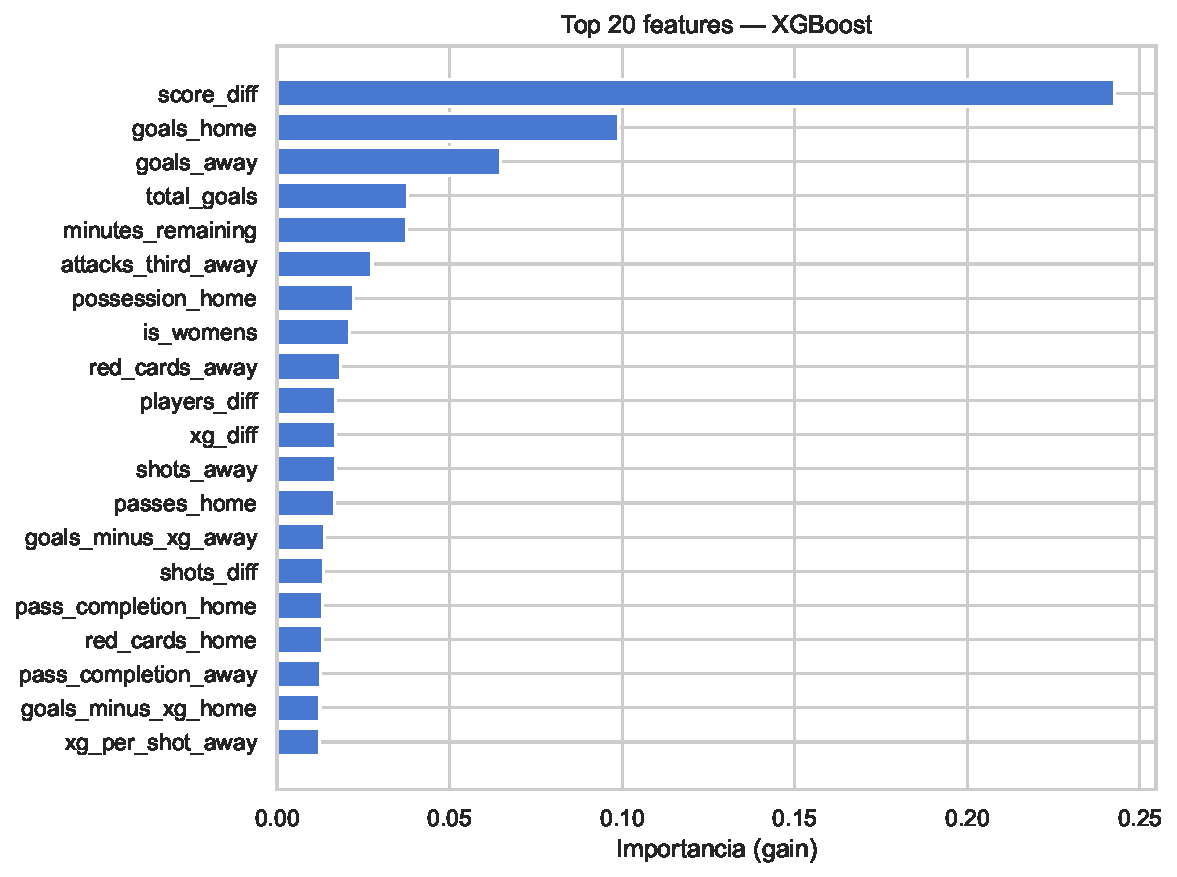
\includegraphics[width=0.80\textwidth]{assets/figuras/modeling/feature_importance_xgb.pdf}
    \caption{Importancia de las 20 variables más relevantes en el XGBoost}
    \label{fig:importancia_xgb}
\end{figure}

\paragraph{SVM lineal}

El SVM lineal obtiene un accuracy global del 63,9 \%, un F1-score macro del 50,0 \% y una pérdida logarítmica de 0,798 sobre el conjunto de test. La tabla \ref{tab:svm_por_minuto} recoge el accuracy y el F1-score macro para los seis puntos de corte evaluados.

\begin{table}[H]
    \centering
    \begin{tabular}{ccc}
        \hline
        \textbf{Minuto} & \textbf{Accuracy} & \textbf{Macro-F1} \\
        \hline
        15              & 56,6 \%           & 42,5 \%           \\
        30              & 60,0 \%           & 45,9 \%           \\
        45              & 63,0 \%           & 48,6 \%           \\
        60              & 68,4 \%           & 54,2 \%           \\
        75              & 70,8 \%           & 56,6 \%           \\
        90              & 77,2 \%           & 65,7 \%           \\
        \hline
    \end{tabular}
    \caption{Accuracy y Macro-F1 del SVM lineal por minuto de partido}
    \label{tab:svm_por_minuto}
\end{table}

El modelo supera el 70 \% de accuracy en el minuto 75, lo que indica que necesita una cantidad elevada de información del partido para alcanzar el umbral de referencia. A diferencia de los modelos basados en árboles, el SVM lineal trabaja con una frontera de decisión más simple, por lo que tiene más dificultad para representar relaciones complejas entre las variables del partido y el resultado final. La figura \ref{fig:svm_minutos} muestra la evolución del accuracy y del F1-score macro por minuto.

\begin{figure}[H]
    \centering
    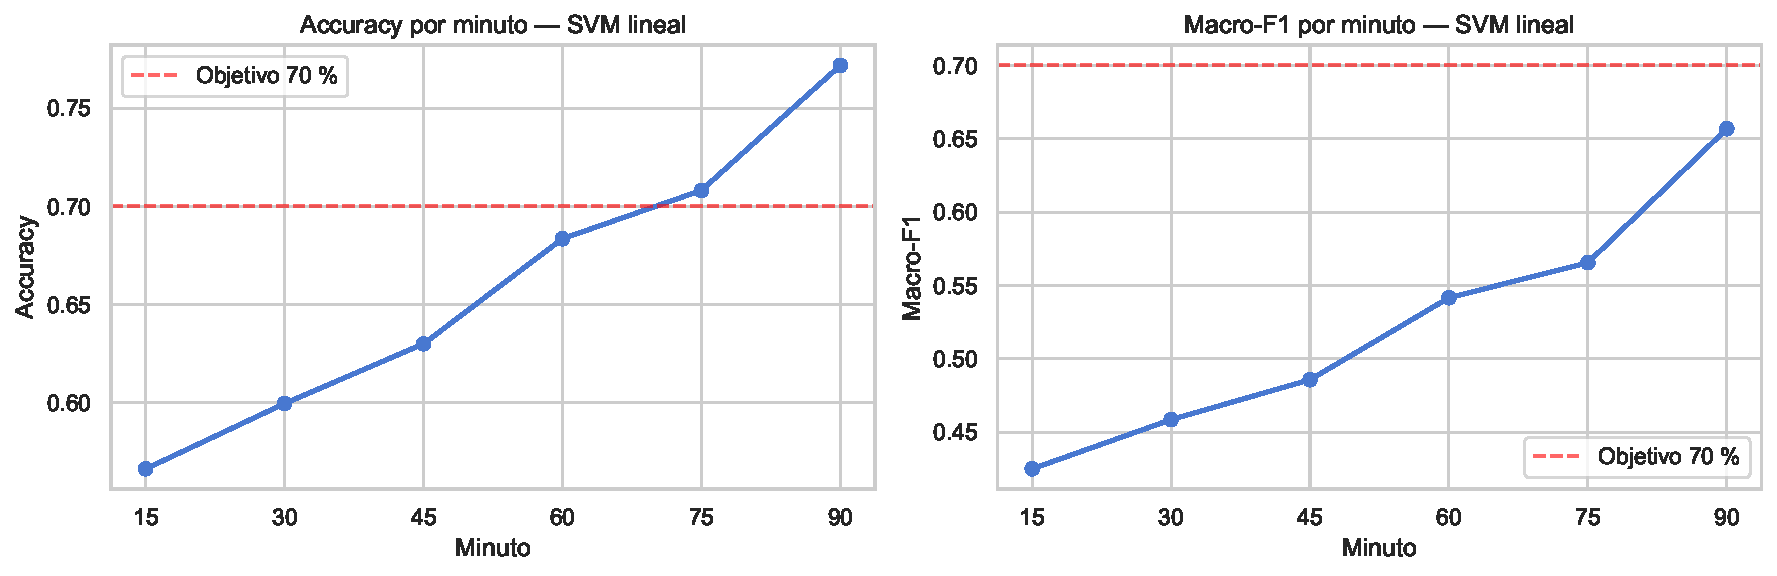
\includegraphics[width=0.95\textwidth]{assets/figuras/modeling/accuracy_por_minuto_svm.pdf}
    \caption{Evolución del accuracy y el Macro-F1 por minuto de partido para el SVM lineal}
    \label{fig:svm_minutos}
\end{figure}

La matriz de confusión normalizada, mostrada en la figura \ref{fig:svm_confusion}, permite observar que el principal problema del modelo se encuentra en la clase empate. Aunque el modelo alcanza resultados razonables para las victorias locales y visitantes, apenas identifica correctamente los empates, con un recall muy bajo para esta clase. Esto afecta directamente al F1-score macro, ya que esta métrica penaliza el mal rendimiento en cualquiera de las clases.

\begin{figure}[H]
    \centering
    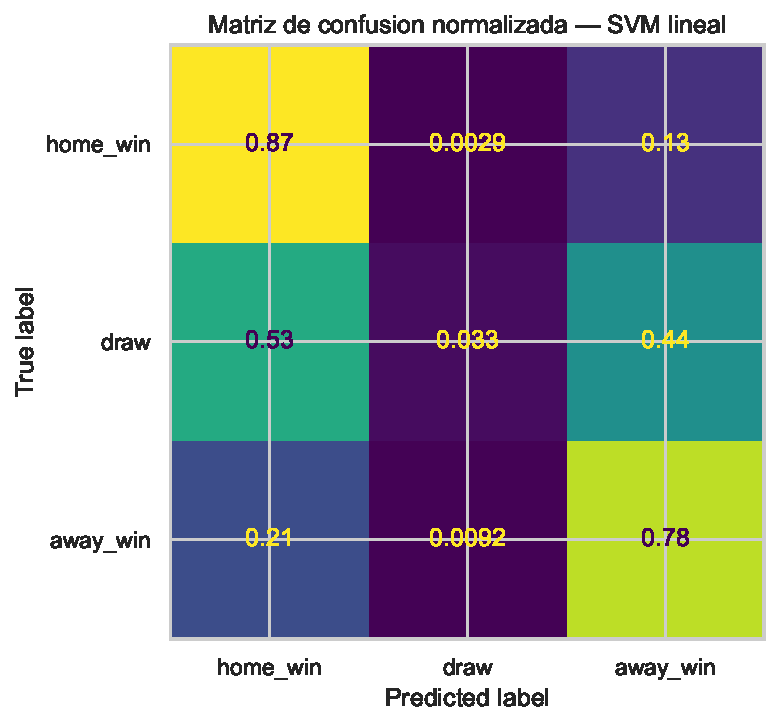
\includegraphics[width=0.65\textwidth]{assets/figuras/modeling/confusion_svm.pdf}
    \caption{Matriz de confusión normalizada del SVM lineal sobre el conjunto de test}
    \label{fig:svm_confusion}
\end{figure}

El análisis de coeficientes del SVM lineal permite obtener una interpretación aproximada de las variables con mayor peso en la decisión del modelo. En este caso, destacan variables relacionadas con la posesión, los pases, la diferencia de goles y el marcador acumulado. No obstante, estos coeficientes deben interpretarse con prudencia, ya que no son directamente equivalentes a las importancias de variables utilizadas en modelos basados en árboles. La figura \ref{fig:svm_coeficientes} muestra las 20 variables con mayor peso medio absoluto en el modelo.

\begin{figure}[H]
    \centering
    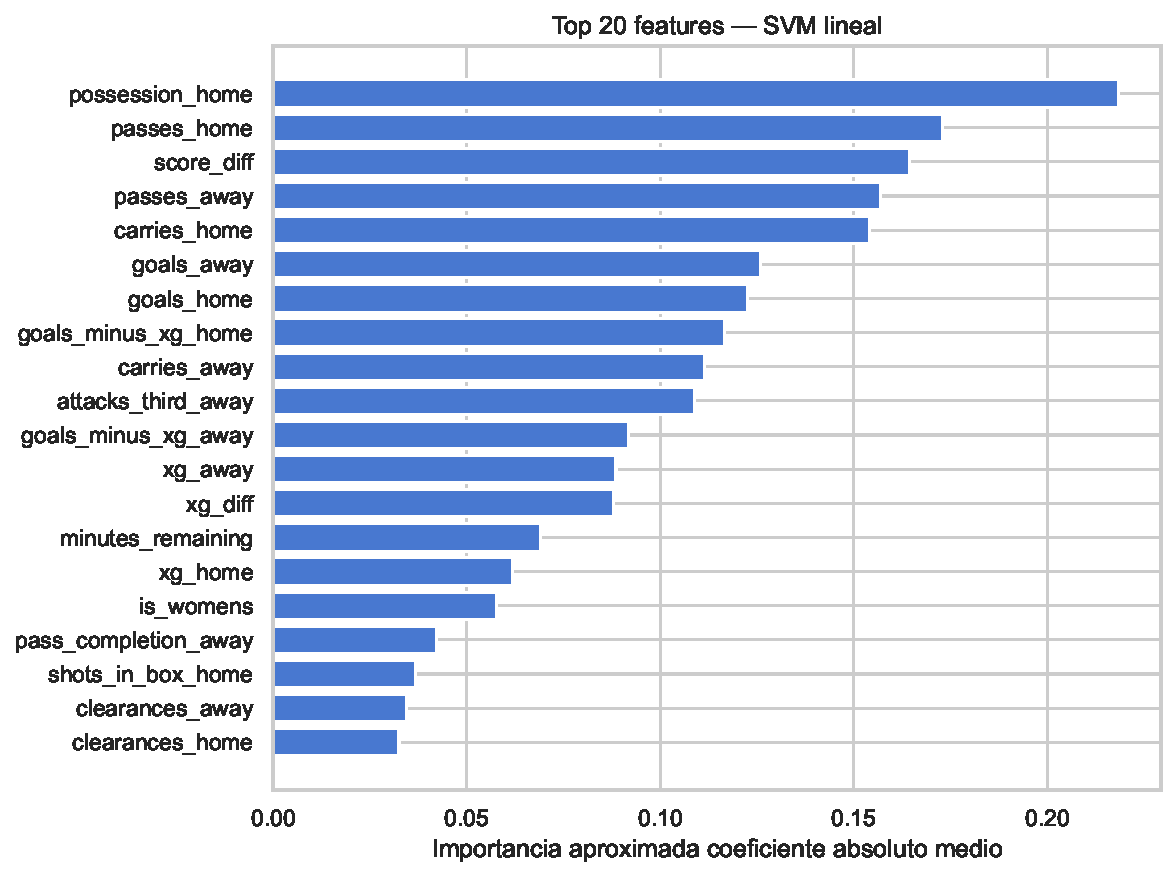
\includegraphics[width=0.85\textwidth]{assets/figuras/modeling/feature_importance_svm.pdf}
    \caption{Coeficientes medios absolutos de las 20 variables más relevantes en el SVM lineal}
    \label{fig:svm_coeficientes}
\end{figure}

\section{Evaluación y despliegue}

\subsection{Evaluación del modelo final}

\subsection{Despliegue}